\documentclass{article}

\usepackage{subcaption}

\usepackage{tikz}

\definecolor{alizarin}{RGB}{231, 76, 60}
\definecolor{pomegranate}{RGB}{192, 57, 43}
\definecolor{emerald}{RGB}{46, 204, 113}
\definecolor{turquoise}{RGB}{26, 188, 156}
\definecolor{greensea}{RGB}{22, 160, 133}

\begin{document}

% FIGURE: horizontal red/green double-opponent cell on horizontal red/green border
\begin{figure}[h]
    \begin{subfigure}{0.3\textwidth}
        \centering
        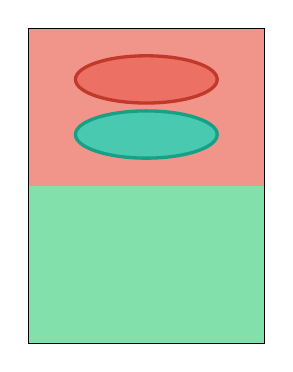
\begin{tikzpicture}
            \fill[alizarin!60]                                         (-1.50, 2.00) rectangle (1.50, 0.00);
            \fill[emerald!60]                                          (-1.50,-2.00) rectangle (1.50, 0.00);
            \filldraw[color=pomegranate, fill=alizarin!80,  very thick]( 0.00, 1.35) ellipse   (0.90 and 0.30);
            \filldraw[color=greensea,    fill=turquoise!80, very thick]( 0.00, 0.65) ellipse   (0.90 and 0.30);
            \draw (current bounding box.north east) rectangle (current bounding box.south west);
        \end{tikzpicture}
        \caption{drawing}
    \end{subfigure}%
    \begin{subfigure}{0.3\textwidth}
        \centering
        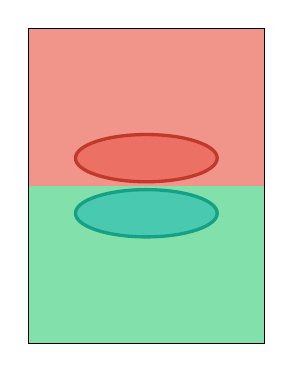
\begin{tikzpicture}
            \fill[alizarin!60]                                         (-1.50, 2.00) rectangle (1.50, 0.00);
            \fill[emerald!60]                                          (-1.50,-2.00) rectangle (1.50, 0.00);
            \filldraw[color=pomegranate, fill=alizarin!80,  very thick]( 0.00, 0.35) ellipse   (0.90 and 0.30);
            \filldraw[color=greensea,    fill=turquoise!80, very thick]( 0.00,-0.35) ellipse   (0.90 and 0.30);
        \draw (current bounding box.north east) rectangle (current bounding box.south west);
        \end{tikzpicture}
        \caption{drawing}
    \end{subfigure}%
    \begin{subfigure}{0.3\textwidth}
        \centering
        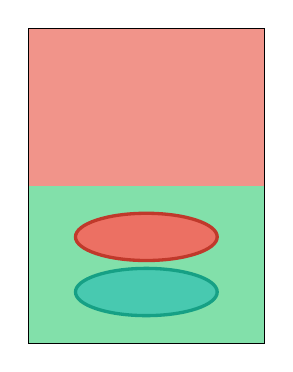
\begin{tikzpicture}
            \fill[alizarin!60]                                         (-1.50, 2.00) rectangle (1.50, 0.00);
            \fill[emerald!60]                                          (-1.50,-2.00) rectangle (1.50, 0.00);
            \filldraw[color=pomegranate, fill=alizarin!80,  very thick]( 0.00,-0.65) ellipse   (0.90 and 0.30);
            \filldraw[color=greensea,    fill=turquoise!80, very thick]( 0.00,-1.35) ellipse   (0.90 and 0.30);
        \draw (current bounding box.north east) rectangle (current bounding box.south west);
        \end{tikzpicture}
        \caption{drawing}
    \end{subfigure}%
    \par \bigskip
    \begin{subfigure}{0.3\textwidth}
        \centering
        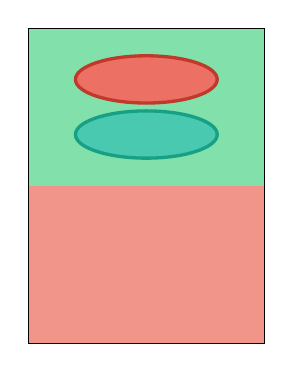
\begin{tikzpicture}
            \fill[emerald!60]                                         (-1.50, 2.00) rectangle (1.50, 0.00);
            \fill[alizarin!60]                                          (-1.50,-2.00) rectangle (1.50, 0.00);
            \filldraw[color=pomegranate, fill=alizarin!80,  very thick]( 0.00, 1.35) ellipse   (0.90 and 0.30);
            \filldraw[color=greensea,    fill=turquoise!80, very thick]( 0.00, 0.65) ellipse   (0.90 and 0.30);
            \draw (current bounding box.north east) rectangle (current bounding box.south west);
        \end{tikzpicture}
        \caption{drawing}
    \end{subfigure}%
    \begin{subfigure}{0.3\textwidth}
        \centering
        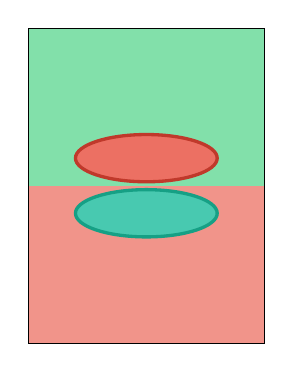
\begin{tikzpicture}
            \fill[emerald!60]                                         (-1.50, 2.00) rectangle (1.50, 0.00);
            \fill[alizarin!60]                                          (-1.50,-2.00) rectangle (1.50, 0.00);
            \filldraw[color=pomegranate, fill=alizarin!80,  very thick]( 0.00, 0.35) ellipse   (0.90 and 0.30);
            \filldraw[color=greensea,    fill=turquoise!80, very thick]( 0.00,-0.35) ellipse   (0.90 and 0.30);
        \draw (current bounding box.north east) rectangle (current bounding box.south west);
        \end{tikzpicture}
        \caption{drawing}
    \end{subfigure}%
    \begin{subfigure}{0.3\textwidth}
        \centering
        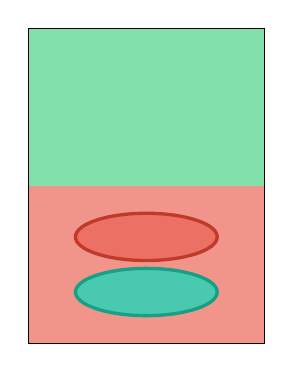
\begin{tikzpicture}
            \fill[emerald!60]                                          (-1.50, 2.00) rectangle (1.50, 0.00);
            \fill[alizarin!60]                                         (-1.50,-2.00) rectangle (1.50, 0.00);
            \filldraw[color=pomegranate, fill=alizarin!80,  very thick]( 0.00,-0.65) ellipse   (0.90 and 0.30);
            \filldraw[color=greensea,    fill=turquoise!80, very thick]( 0.00,-1.35) ellipse   (0.90 and 0.30);
        \draw (current bounding box.north east) rectangle (current bounding box.south west);
        \end{tikzpicture}
        \caption{drawing}
    \end{subfigure}
\end{figure}

The following figure is different
% FIGURE: vertical red/green double-opponent cell on horizontal red/green border
\begin{figure}[h]
    \begin{subfigure}{0.3\textwidth}
        \centering
        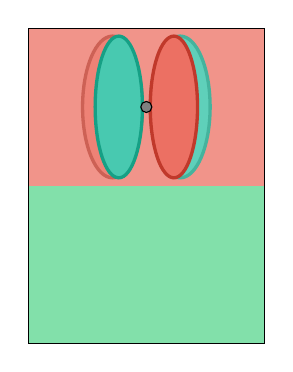
\begin{tikzpicture}
            \fill[alizarin!60]                                            (-1.50, 2.00) rectangle (1.50, 0.00);
            \fill[emerald!60]                                             (-1.50,-2.00) rectangle (1.50, 0.00);
            \filldraw[color=greensea!80,    fill=turquoise!70, very thick]( 0.43, 1.00) ellipse   (0.38 and 0.90);
            \filldraw[color=pomegranate!80, fill=alizarin!70,  very thick](-0.43, 1.00) ellipse   (0.38 and 0.90);
            \filldraw[color=pomegranate,    fill=alizarin!80,  very thick]( 0.35, 1.00) ellipse   (0.30 and 0.90);
            \filldraw[color=greensea,       fill=turquoise!80, very thick](-0.35, 1.00) ellipse   (0.30 and 0.90);
            \filldraw[color=black, fill=gray]                             ( 0.00, 1.00) circle    (2pt);
            \draw (current bounding box.north east) rectangle (current bounding box.south west);
        \end{tikzpicture}
        \caption{Response = 0}
    \end{subfigure}%
    \begin{subfigure}{0.3\textwidth}
        \centering
            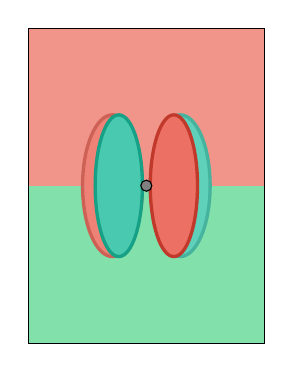
\begin{tikzpicture}
            \fill[alizarin!60]                                            (-1.50, 2.00) rectangle (1.50, 0.00);
            \fill[emerald!60]                                             (-1.50,-2.00) rectangle (1.50, 0.00);
            \filldraw[color=greensea!80,    fill=turquoise!70, very thick]( 0.43, 0.00) ellipse   (0.38 and 0.90);
            \filldraw[color=pomegranate!80, fill=alizarin!70,  very thick](-0.43, 0.00) ellipse   (0.38 and 0.90);
            \filldraw[color=pomegranate,    fill=alizarin!80,  very thick]( 0.35, 0.00) ellipse   (0.30 and 0.90);
            \filldraw[color=greensea,       fill=turquoise!80, very thick](-0.35, 0.00) ellipse   (0.30 and 0.90);
            \filldraw[color=black, fill=gray]                             ( 0.00, 0.00) circle    (2pt);
            \draw (current bounding box.north east) rectangle (current bounding box.south west);
            \end{tikzpicture}
        \caption{Response = 0}
    \end{subfigure}%
    \begin{subfigure}{0.3\textwidth}
        \centering
            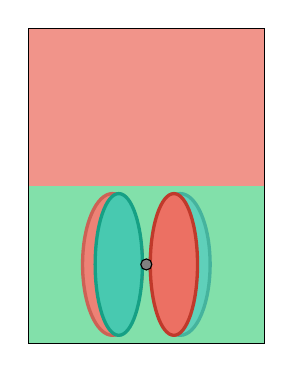
\begin{tikzpicture}
            \fill[alizarin!60]                                            (-1.50, 2.00) rectangle (1.50, 0.00);
            \fill[emerald!60]                                             (-1.50,-2.00) rectangle (1.50, 0.00);
            \filldraw[color=greensea!80,    fill=turquoise!70, very thick]( 0.43,-1.00) ellipse   (0.38 and 0.90);
            \filldraw[color=pomegranate!80, fill=alizarin!70,  very thick](-0.43,-1.00) ellipse   (0.38 and 0.90);
            \filldraw[color=pomegranate,    fill=alizarin!80,  very thick]( 0.35,-1.00) ellipse   (0.30 and 0.90);
            \filldraw[color=greensea,       fill=turquoise!80, very thick](-0.35,-1.00) ellipse   (0.30 and 0.90);
            \filldraw[color=black, fill=gray]                             ( 0.00,-1.00) circle    (2pt);
            \draw (current bounding box.north east) rectangle (current bounding box.south west);
            \end{tikzpicture}
        \caption{Response = 0}
    \end{subfigure}%
    \par \bigskip
    \begin{subfigure}{0.3\textwidth}
        \centering
        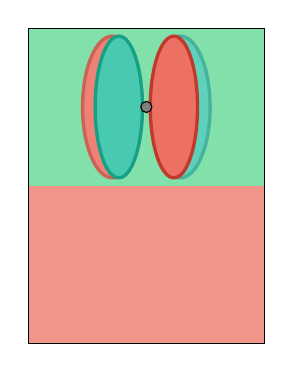
\begin{tikzpicture}
            \fill[emerald!60]                                             (-1.50, 2.00) rectangle (1.50, 0.00);
            \fill[alizarin!60]                                            (-1.50,-2.00) rectangle (1.50, 0.00);
            \filldraw[color=greensea!80,    fill=turquoise!70, very thick]( 0.43, 1.00) ellipse   (0.38 and 0.90);
            \filldraw[color=pomegranate!80, fill=alizarin!70,  very thick](-0.43, 1.00) ellipse   (0.38 and 0.90);
            \filldraw[color=pomegranate,    fill=alizarin!80,  very thick]( 0.35, 1.00) ellipse   (0.30 and 0.90);
            \filldraw[color=greensea,       fill=turquoise!80, very thick](-0.35, 1.00) ellipse   (0.30 and 0.90);
            \filldraw[color=black, fill=gray]                             ( 0.00, 1.00) circle    (2pt);
            \draw (current bounding box.north east) rectangle (current bounding box.south west);
        \end{tikzpicture}
        \caption{Response = 0}
    \end{subfigure}%
    \begin{subfigure}{0.3\textwidth}
        \centering
            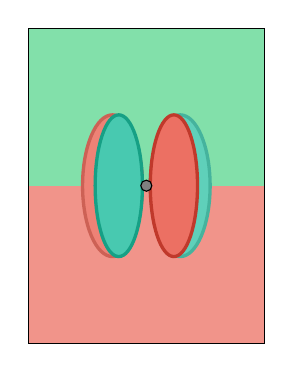
\begin{tikzpicture}
            \fill[emerald!60]                                             (-1.50, 2.00) rectangle (1.50, 0.00);
            \fill[alizarin!60]                                            (-1.50,-2.00) rectangle (1.50, 0.00);
            \filldraw[color=greensea!80,    fill=turquoise!70, very thick]( 0.43, 0.00) ellipse   (0.38 and 0.90);
            \filldraw[color=pomegranate!80, fill=alizarin!70,  very thick](-0.43, 0.00) ellipse   (0.38 and 0.90);
            \filldraw[color=pomegranate,    fill=alizarin!80,  very thick]( 0.35, 0.00) ellipse   (0.30 and 0.90);
            \filldraw[color=greensea,       fill=turquoise!80, very thick](-0.35, 0.00) ellipse   (0.30 and 0.90);
            \filldraw[color=black, fill=gray]                             ( 0.00, 0.00) circle    (2pt);
            \draw (current bounding box.north east) rectangle (current bounding box.south west);
            \end{tikzpicture}
        \caption{Response = 0}
    \end{subfigure}%
    \begin{subfigure}{0.3\textwidth}
        \centering
            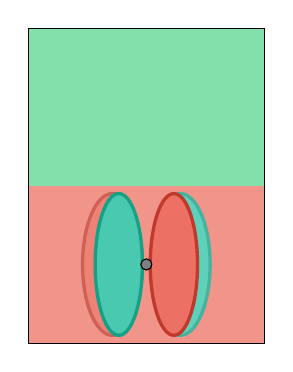
\begin{tikzpicture}
            \fill[emerald!60]                                             (-1.50, 2.00) rectangle (1.50, 0.00);
            \fill[alizarin!60]                                            (-1.50,-2.00) rectangle (1.50, 0.00);
            \filldraw[color=greensea!80,    fill=turquoise!70, very thick]( 0.43,-1.00) ellipse   (0.38 and 0.90);
            \filldraw[color=pomegranate!80, fill=alizarin!70,  very thick](-0.43,-1.00) ellipse   (0.38 and 0.90);
            \filldraw[color=pomegranate,    fill=alizarin!80,  very thick]( 0.35,-1.00) ellipse   (0.30 and 0.90);
            \filldraw[color=greensea,       fill=turquoise!80, very thick](-0.35,-1.00) ellipse   (0.30 and 0.90);
            \filldraw[color=black, fill=gray]                             ( 0.00,-1.00) circle    (2pt);
            \draw (current bounding box.north east) rectangle (current bounding box.south west);
            \end{tikzpicture}
        \caption{Response = 0}
    \end{subfigure}
    \caption{A double opponent cell selective to vertically oriented borders; completely unresponsive to a horizontal border. While itss $R_{on}$ receptive field might be strongly stimulated in (a) and (f), it's $R_{off}$ receptive field cancels it out. Similarly, in (c) and (d) its $G_{on}$ receptive field is stimulated but cancelled out by activity in its $G_{off}$ receptive field. In (b) and (e) both of its $R_{on}$ and $G_{on}$ receptive fields are moderately activated, but again, cancelled out by activation in its $R_{off}$ and $G_{off}$ receptive fields, respectively.}
\end{figure}

\end{document}